% --- ETUDE DE CAS ---
\newpage

\section*{AAV}
\addcontentsline{toc}{section}{AAV}
\begin{itemize}
	\item [1] Citer les bonnes pratiques de déploiement d’API REST en utilisant Node.js
	\item [1] Citer les différents types d’infrastructures de déploiement
	\item [3] Définir les propriétés non fonctionnelles (fiabilité, performance, disponibilité, scalabilité, connectivité, évolutivité)
	\item [6] Expliquer l'utilisation d'un ORM Java-Script
	\item [3] Expliquer les possibilités d’architecture logicielle adaptée pour le projet (monolithiques -> Microservices)
	\item [3] Représenter l'architecture logicielle retenue de manière argumentée
\end{itemize}

\newpage

\section*{Étude de cas~: API}
\addcontentsline{toc}{section}{Étude de cas~: API}

\subsection*{Mots clés}
\phantomsection
\addcontentsline{toc}{subsection}{Mots clés}
\begin{itemize}
	\item Migration en MSA
	\item Full Stack
	\item Application monolithique
	\item Architecture en micro-services
	\item API REST
	\item pile MERN
	\item EKS
	\item AWS
	\item Orchestrateur
	\item ODM (Mongoose)
	\item Nginx
	\item MongoDB
	\item CRUD
	\item API Gateway
	\item Docker (container)
	\item Scalability
	\item CICD
	\item Maturité de Richardson
\end{itemize}

\subsection*{Contexte}
\phantomsection
\addcontentsline{toc}{subsection}{Contexte}
\noindent L’entreprise souhaite migrer progressivement son application monolithique vers une architecture en microservices. Le réseau social intégré à l’application de lecture et vente de bandes dessinées est utilisé comme projet pilote afin de développer un service backend exposant une API REST avec Node.js, Express et MongoDB.

\subsection*{Problématique}
\phantomsection
\addcontentsline{toc}{subsection}{Problématique}
\noindent Comment concevoir une API REST, scalable et intégrable dans une architecture microservices tout en garantissant la séparation des services, la conteneurisation et la compatibilité avec une future infrastructure cloud ?

\subsection*{Contraintes}
\phantomsection
\addcontentsline{toc}{subsection}{Contraintes}
\begin{itemize}
	\item Node.js
	\item Express
	\item MongoDB
	\item Mongoose
	\item Niveau de maturité 2 (API)
	\item Docker
	\item Scalabilité
	\item API Gateway
	\item Load balancer Nginx
\end{itemize}

\subsection*{Généralisation}
\phantomsection
\addcontentsline{toc}{subsection}{Généralisation}
\begin{itemize}
	\item API REST
	\item Microservices
	\item Conteneurisation
	\item Scalabilité
	\item Déploiement continu
	\item Persistance NoSQL
\end{itemize}

\subsection*{Livrables}
\phantomsection
\addcontentsline{toc}{subsection}{Livrables}
\begin{itemize}
	\item Prototype CRUD gestion des posts
	\item Architecture logicielle documentée
	\item Exemples de bonnes pratiques de déploiement Docker
\end{itemize}

\newpage

\subsection*{Pistes de solutions}
\phantomsection
\addcontentsline{toc}{subsection}{Pistes de solutions}
\begin{itemize}
	\item Architecture microservices avec Node.js et Express
	\item Les API REST pour la communication entre services
	\item Utilisation de MongoDB pour la persistance des données
	\item Conteneurisation avec Docker pour faciliter le déploiement
	\item Modèle Client-Serveur pour structurer les interactions
\end{itemize}

\subsection*{Plan d'actions}
\phantomsection
\addcontentsline{toc}{subsection}{Plan d'actions}
\begin{itemize}
	\item Définir les mots clés
	\item Etudier les principes de l'architecture microservices et des API REST
	\item Concevoir une architecture logicielle adaptée au projet
	\item Implémenter un prototype CRUD pour la gestion des posts
	\item Documenter l'architecture logicielle retenue
	\item Présenter des exemples de bonnes pratiques de déploiement avec Docker
\end{itemize}

\newpage

\section*{Définition~: Mots clés}
\phantomsection
\addcontentsline{toc}{section}{Définition~: Mots clés}

\subsubsection*{Migration en MSA}
\phantomsection
\addcontentsline{toc}{subsection}{Migration en MSA}

La \textit{Migration en MSA} (\textit{MicroServices Architecture}) désigne le processus consistant à faire évoluer une application existante, généralement \textbf{monolithique}, vers une \textbf{architecture en micro-services}. Plutôt que de tout réécrire d'un seul bloc (approche risquée dite \og{}Big Bang\fg{}), la migration est presque toujours \textbf{progressive}~: on extrait un à un les modules métiers du monolithe pour en faire des services indépendants. Le \textit{pattern} de référence est le \og{}\textit{Strangler Fig}\fg{} (figure de l'étrangleur)~: les nouvelles fonctionnalités sont développées en micro-services tandis que l'ancien code est peu à peu \og{}étranglé\fg{}, jusqu'à disparaître. Dans le projet, le réseau social de l'application BD sert de \textbf{projet pilote}~: c'est le premier domaine métier extrait du monolithe pour valider la démarche avant de l'étendre au reste de l'application.

\vspace{0.4cm}

\subsubsection*{Full Stack}
\phantomsection
\addcontentsline{toc}{subsection}{Full Stack}

\noindent Le terme \textit{Full Stack} qualifie un développement (ou un développeur) couvrant l'\textbf{ensemble de la pile technique} d'une application, du \textbf{front-end} au \textbf{back-end} en passant par la base de données et le déploiement. On distingue trois couches~:
\begin{itemize}
	\item \textbf{Front-end} (client)~: la partie visible, exécutée dans le navigateur (HTML, CSS, JavaScript, ici React).
	\item \textbf{Back-end} (serveur)~: la logique métier et l'API (ici Node.js + Express).
	\item \textbf{Base de données}~: la persistance des données (ici MongoDB).
\end{itemize}
\noindent La \textbf{pile MERN} (voir plus bas) est précisément une stack \textit{Full Stack} où un seul langage, le JavaScript, est utilisé sur les trois couches, ce qui simplifie le développement et le partage de compétences.

\newpage

\subsubsection*{Application monolithique}
\phantomsection
\addcontentsline{toc}{subsection}{Application monolithique}

Une \textit{application monolithique} est une application construite comme un \textbf{bloc unique et indivisible}~: l'interface, la logique métier et l'accès aux données sont regroupés dans une seule base de code, compilée et déployée d'un seul tenant. Tous les modules partagent le même processus et, souvent, la même base de données.

\noindent \textbf{Avantages}~: simplicité initiale, déploiement unique, communication interne rapide (appels de fonctions en mémoire). \textbf{Inconvénients}~: couplage fort entre modules, montée en charge difficile (on doit dupliquer toute l'application même si un seul module est sollicité), une panne peut faire tomber l'ensemble, et tout changement impose de re-déployer la totalité — ce qui freine l'\textbf{évolutivité} et l'agilité des équipes. C'est précisément ce qui motive la migration vers les micro-services.

\begin{center}
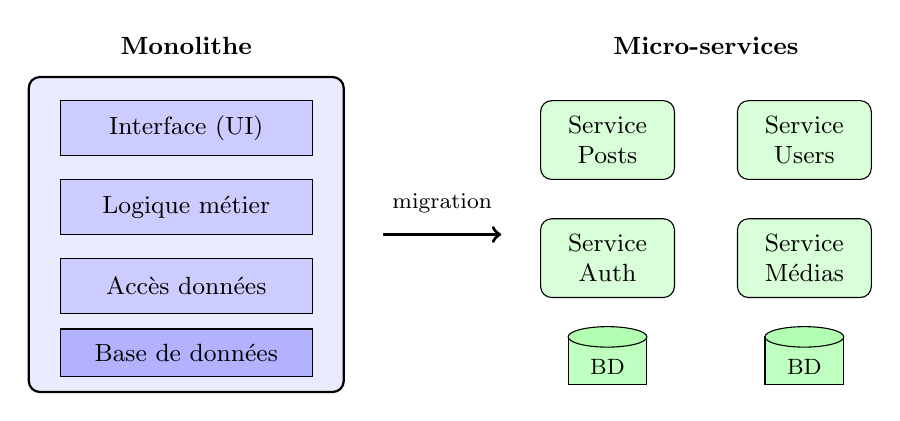
\begin{tikzpicture}[font=\small]
	% --- Monolithe ---
	\draw[thick, fill=blue!8, rounded corners] (0,0) rectangle (4,4);
	\node at (2,4.4) {\textbf{Monolithe}};
	\draw[fill=blue!20] (0.4,3.0) rectangle (3.6,3.7) node[midway]{Interface (UI)};
	\draw[fill=blue!20] (0.4,2.0) rectangle (3.6,2.7) node[midway]{Logique métier};
	\draw[fill=blue!20] (0.4,1.0) rectangle (3.6,1.7) node[midway]{Accès données};
	\draw[fill=blue!30] (0.4,0.2) rectangle (3.6,0.8) node[midway]{Base de données};

	% --- Fleche ---
	\draw[->, very thick] (4.5,2) -- (6.0,2);
	\node at (5.25,2.4) {\footnotesize migration};

	% --- Microservices ---
	\node at (8.6,4.4) {\textbf{Micro-services}};
	\draw[fill=green!15, rounded corners] (6.5,2.7) rectangle (8.2,3.7) node[midway, align=center]{Service\\Posts};
	\draw[fill=green!15, rounded corners] (9.0,2.7) rectangle (10.7,3.7) node[midway, align=center]{Service\\Users};
	\draw[fill=green!15, rounded corners] (6.5,1.2) rectangle (8.2,2.2) node[midway, align=center]{Service\\Auth};
	\draw[fill=green!15, rounded corners] (9.0,1.2) rectangle (10.7,2.2) node[midway, align=center]{Service\\Médias};
	\draw[fill=green!25] (6.85,0.1) rectangle (7.85,0.7);
	\draw[fill=green!30] (7.35,0.7) ellipse (0.5 and 0.13);
	\node at (7.35,0.32) {\footnotesize BD};
	\draw[fill=green!25] (9.35,0.1) rectangle (10.35,0.7);
	\draw[fill=green!30] (9.85,0.7) ellipse (0.5 and 0.13);
	\node at (9.85,0.32) {\footnotesize BD};
\end{tikzpicture}
\end{center}

\noindent\textit{Figure~: du bloc monolithique unique vers des services indépendants disposant chacun de sa propre base de données.}

\vspace{0.4cm}

\subsubsection*{Architecture en micro-services}
\phantomsection
\addcontentsline{toc}{subsection}{Architecture en micro-services}

L'\textit{architecture en micro-services} (MSA) consiste à découper une application en un ensemble de \textbf{petits services autonomes}, chacun responsable d'une seule capacité métier (gestion des posts, des utilisateurs, de l'authentification, etc.). Chaque service~:
\begin{itemize}
	\item est \textbf{développé, déployé et mis à l'échelle indépendamment} des autres~;
	\item possède idéalement sa \textbf{propre base de données} (\textit{Database per Service})~;
	\item communique avec les autres via des \textbf{interfaces réseau légères}, le plus souvent des \textbf{API REST} en HTTP/JSON.
\end{itemize}
\noindent \textbf{Avantages}~: \textbf{scalabilité} fine (on ne met à l'échelle que le service sollicité), \textbf{résilience} (une panne reste isolée), liberté technologique par service, déploiements indépendants et plus fréquents (\textbf{évolutivité}). \textbf{Inconvénients}~: complexité accrue (réseau, supervision, cohérence des données distribuées), nécessité d'outils d'orchestration et d'une \textbf{API Gateway}.

\newpage

\subsubsection*{API REST}
\phantomsection
\addcontentsline{toc}{subsection}{API REST}

Une \textbf{API} (\textit{Application Programming Interface}) est un contrat qui permet à deux logiciels de dialoguer. \textbf{REST} (\textit{REpresentational State Transfer}) est un \textbf{style d'architecture} pour concevoir des API au-dessus du protocole \textbf{HTTP}. Une API REST manipule des \textbf{ressources} (ex.~: un \textit{post}, un \textit{user}) identifiées par des \textbf{URI} (ex.~: \texttt{/api/posts/42}), sur lesquelles on applique les \textbf{verbes HTTP}~:

\vspace{0.2cm}

\begin{center}
\begin{tabular}{|l|l|l|}
\hline
\textbf{Verbe HTTP} & \textbf{Action CRUD} & \textbf{Exemple} \\ \hline
GET    & Lire (Read)      & \texttt{GET /api/posts} \\ \hline
POST   & Créer (Create)   & \texttt{POST /api/posts} \\ \hline
PUT / PATCH & Mettre à jour (Update) & \texttt{PUT /api/posts/42} \\ \hline
DELETE & Supprimer (Delete) & \texttt{DELETE /api/posts/42} \\ \hline
\end{tabular}
\end{center}
\vspace{0.2cm}

\noindent Les principes clés de REST sont~: l'architecture \textbf{Client-Serveur}, le caractère \textbf{sans état} (\textit{stateless}~: chaque requête contient toute l'information nécessaire, le serveur ne mémorise pas la session), une \textbf{interface uniforme}, et l'échange de représentations standardisées (généralement du \textbf{JSON}).

\begin{center}
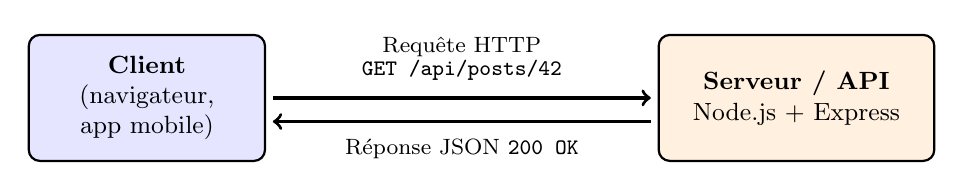
\begin{tikzpicture}[font=\small]
	\draw[thick, fill=blue!10, rounded corners] (0,0.4) rectangle (3,2) node[midway, align=center]{\textbf{Client}\\(navigateur,\\app mobile)};
	\draw[thick, fill=orange!12, rounded corners] (8,0.4) rectangle (11.5,2) node[midway, align=center]{\textbf{Serveur / API}\\Node.js + Express};
	\draw[->, very thick] (3.1,1.2) -- (7.9,1.2);
	\node[align=center] at (5.5,1.85) {\footnotesize Requête HTTP};
	\node[align=center] at (5.5,1.55) {\footnotesize \texttt{GET /api/posts/42}};
	\draw[<-, very thick] (3.1,0.9) -- (7.9,0.9);
	\node[align=center] at (5.5,0.55) {\footnotesize Réponse JSON \texttt{200 OK}};
\end{tikzpicture}
\end{center}
\noindent\textit{Figure~: échange Client-Serveur sans état au cœur d'une API REST.}

\vspace{0.4cm}

\subsubsection*{Pile MERN}
\phantomsection
\addcontentsline{toc}{subsection}{Pile MERN}

La \textbf{pile MERN} est un ensemble de quatre technologies \textbf{tout-JavaScript} permettant de construire une application web \textit{Full Stack}~:
\begin{itemize}
	\item \textbf{M -- MongoDB}~: base de données NoSQL orientée documents (persistance).
	\item \textbf{E -- Express}~: framework web minimaliste pour Node.js (routes et API REST).
	\item \textbf{R -- React}~: bibliothèque front-end pour l'interface utilisateur (côté client).
	\item \textbf{N -- Node.js}~: environnement d'exécution JavaScript côté serveur.
\end{itemize}
\noindent Son intérêt majeur~: un \textbf{langage unique (JavaScript)} de bout en bout, et un format de données homogène (\textbf{JSON / BSON}) du navigateur jusqu'à la base, ce qui réduit les frictions et facilite le travail des équipes \textit{Full Stack}.

\newpage

\subsubsection*{EKS}
\phantomsection
\addcontentsline{toc}{subsection}{EKS}

\textbf{EKS} (\textit{Elastic Kubernetes Service}) est le service \textbf{managé Kubernetes} proposé par \textbf{AWS}. Il fournit un cluster \textbf{Kubernetes} (l'orchestrateur de référence) dont AWS gère pour nous le \textit{control plane} (le \og{}cerveau\fg{} qui pilote les conteneurs), la haute disponibilité et les mises à jour. EKS permet de \textbf{déployer, orchestrer et mettre à l'échelle} automatiquement des conteneurs Docker dans le \textbf{cloud}. Dans le contexte du projet, EKS représente l'\textbf{infrastructure cible} permettant d'héberger les micro-services conteneurisés de façon scalable et résiliente.

\vspace{0.4cm}

\subsubsection*{AWS}
\phantomsection
\addcontentsline{toc}{subsection}{AWS}

\textbf{AWS} (\textit{Amazon Web Services}) est la plateforme de \textbf{cloud computing} d'Amazon, leader du marché. Elle propose, à la demande et facturé à l'usage (\textit{pay-as-you-go}), une vaste gamme de services~: \textbf{calcul} (EC2), \textbf{conteneurs/orchestration} (ECS, \textbf{EKS}), \textbf{stockage} (S3), \textbf{bases de données}, \textbf{réseau} et \textbf{équilibrage de charge}. AWS illustre l'\textbf{infrastructure de type IaaS/PaaS} (\og{}cloud public\fg{}) vers laquelle le projet doit rester compatible, par opposition à un hébergement \og{}on-premise\fg{} (sur les serveurs de l'entreprise).

\vspace{0.4cm}

\subsubsection*{Orchestrateur}
\phantomsection
\addcontentsline{toc}{subsection}{Orchestrateur}

Un \textbf{orchestrateur} de conteneurs est un outil qui \textbf{automatise le déploiement, la gestion, la mise à l'échelle et le réseau} d'un grand nombre de conteneurs. Là où Docker lance un conteneur, l'orchestrateur gère une \textbf{flotte} de conteneurs répartis sur plusieurs machines. Le standard du marché est \textbf{Kubernetes} (souvent abrégé \textbf{K8s}). Ses fonctions principales~:
\begin{itemize}
	\item \textbf{Scaling automatique}~: ajout/retrait de conteneurs selon la charge.
	\item \textbf{Auto-réparation}~: redémarre un conteneur défaillant (\textbf{fiabilité / disponibilité}).
	\item \textbf{Load balancing}~: répartit le trafic entre les instances.
	\item \textbf{Déploiements progressifs} (\textit{rolling updates}) sans interruption de service.
\end{itemize}
\noindent C'est l'élément indispensable pour exploiter une architecture micro-services à grande échelle (cf. \textbf{EKS}).

\newpage

\subsubsection*{ODM (Mongoose)}
\phantomsection
\addcontentsline{toc}{subsection}{ODM (Mongoose)}

Un \textbf{ODM} (\textit{Object-Document Mapping}) est l'équivalent d'un \textbf{ORM} (\textit{Object-Relational Mapping}) mais pour les bases \textbf{NoSQL orientées documents} comme MongoDB. Il fait le pont entre le \textbf{monde objet} du code (objets JavaScript) et les \textbf{documents} stockés en base, évitant d'écrire des requêtes bas niveau.

\noindent \textbf{Mongoose} est l'ODM de référence pour MongoDB en Node.js. Il apporte~:
\begin{itemize}
	\item des \textbf{Schémas} qui définissent la structure et les types des documents~;
	\item une \textbf{validation} automatique des données avant insertion~;
	\item des \textbf{modèles} offrant des méthodes CRUD prêtes à l'emploi (\texttt{find}, \texttt{create}, ...)~;
	\item la gestion des relations, des \textit{hooks} et des requêtes typées.
\end{itemize}
\noindent C'est l'illustration directe de l'AAV \og{}Expliquer l'utilisation d'un ORM JavaScript\fg{}~: Mongoose abstrait l'accès aux données, fiabilise le code et accélère le développement.

\vspace{0.5cm}

\subsubsection*{Nginx}
\phantomsection
\addcontentsline{toc}{subsection}{Nginx}

\textbf{Nginx} (prononcé \og{}engine-x\fg{}) est un \textbf{serveur web} hautes performances qui joue, dans une architecture distribuée, deux rôles essentiels~:
\begin{itemize}
	\item \textbf{Reverse proxy}~: il se place devant les serveurs applicatifs et reçoit les requêtes des clients pour les transmettre aux bons services (point d'entrée unique, terminaison TLS/HTTPS).
	\item \textbf{Load balancer} (équilibreur de charge)~: il \textbf{répartit le trafic} entre plusieurs instances d'un même service, ce qui améliore la \textbf{performance}, la \textbf{disponibilité} et permet la \textbf{scalabilité horizontale}.
\end{itemize}
\begin{center}
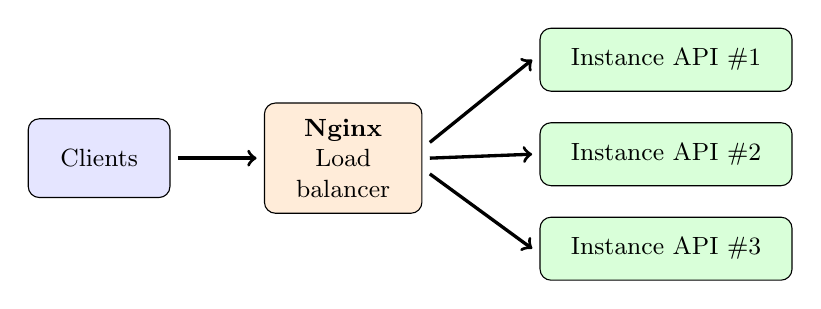
\begin{tikzpicture}[font=\small]
	\draw[fill=blue!10, rounded corners] (0,1) rectangle (1.8,2) node[midway]{Clients};
	\draw[fill=orange!15, rounded corners] (3,0.8) rectangle (5,2.2) node[midway, align=center]{\textbf{Nginx}\\Load\\balancer};
	\draw[->, very thick] (1.9,1.5) -- (2.9,1.5);
	\draw[fill=green!15, rounded corners] (6.5,2.35) rectangle (9.7,3.15) node[midway]{Instance API \#1};
	\draw[fill=green!15, rounded corners] (6.5,1.15) rectangle (9.7,1.95) node[midway]{Instance API \#2};
	\draw[fill=green!15, rounded corners] (6.5,-0.05) rectangle (9.7,0.75) node[midway]{Instance API \#3};
	\draw[->, very thick] (5.1,1.7) -- (6.4,2.75);
	\draw[->, very thick] (5.1,1.5) -- (6.4,1.55);
	\draw[->, very thick] (5.1,1.3) -- (6.4,0.35);
\end{tikzpicture}
\end{center}
\noindent\textit{Figure~: Nginx répartit la charge entre plusieurs instances de l'API (scalabilité horizontale).}

\newpage

\subsubsection*{MongoDB}
\phantomsection
\addcontentsline{toc}{subsection}{MongoDB}

\textbf{MongoDB} est un \textbf{système de gestion de base de données NoSQL} orienté \textbf{documents}. Au lieu de tables et de lignes (modèle relationnel), il stocke les données sous forme de \textbf{documents JSON/BSON} flexibles, regroupés en \textbf{collections}. Exemple d'un document \textit{post}~:
\begin{center}
\texttt{\{ "\_id": 42, "auteur": "Alice", "contenu": "...", "likes": 12 \}}
\end{center}
\noindent \textbf{Atouts}~: \textbf{schéma flexible} (idéal pour des données évolutives), excellente \textbf{scalabilité horizontale} (\textit{sharding}), bonnes performances en lecture/écriture, et homogénéité avec JavaScript (format JSON). C'est le \og{}M\fg{} de la pile \textbf{MERN} et la solution de \textbf{persistance NoSQL} retenue, avec un principe \textit{Database per Service} dans l'architecture micro-services.

\vspace{0.4cm}

\subsubsection*{CRUD}
\phantomsection
\addcontentsline{toc}{subsection}{CRUD}

\textbf{CRUD} est l'acronyme des \textbf{quatre opérations fondamentales} de manipulation de données persistées~:
\begin{itemize}
	\item \textbf{C -- Create} (créer) — \texttt{POST}
	\item \textbf{R -- Read} (lire) — \texttt{GET}
	\item \textbf{U -- Update} (mettre à jour) — \texttt{PUT/PATCH}
	\item \textbf{D -- Delete} (supprimer) — \texttt{DELETE}
\end{itemize}
\noindent Ces opérations correspondent directement aux \textbf{verbes HTTP} d'une API REST et aux méthodes d'un ODM comme Mongoose. Le \textbf{livrable du projet} est précisément un \textbf{prototype CRUD de gestion des posts} du réseau social.

\newpage

\subsubsection*{API Gateway}
\phantomsection
\addcontentsline{toc}{subsection}{API Gateway}

Une \textbf{API Gateway} (passerelle d'API) est le \textbf{point d'entrée unique} d'une architecture micro-services. Tous les appels clients passent par elle, et elle se charge de les \textbf{router} vers le bon micro-service. Elle centralise des préoccupations transverses qu'il serait coûteux de dupliquer dans chaque service~:
\begin{itemize}
	\item \textbf{routage} et agrégation des requêtes~;
	\item \textbf{authentification / autorisation} (ex.~: vérification des jetons JWT)~;
	\item \textbf{limitation de débit} (\textit{rate limiting}), journalisation, mise en cache~;
	\item \textbf{terminaison TLS} et masquage de la structure interne (\textbf{connectivité} simplifiée pour le client).
\end{itemize}
\begin{center}
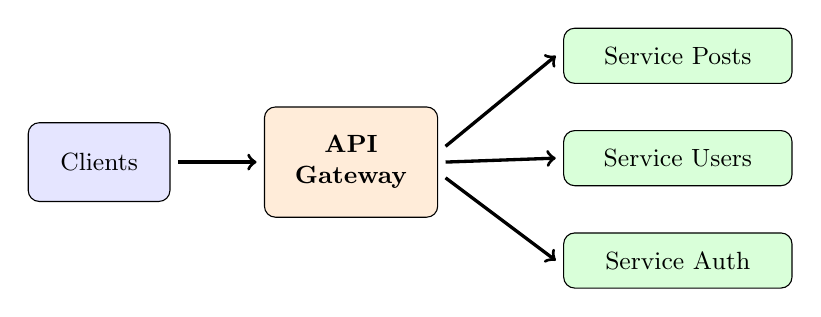
\begin{tikzpicture}[font=\small]
	\draw[fill=blue!10, rounded corners] (0,0.8) rectangle (1.8,1.8) node[midway]{Clients};
	\draw[fill=orange!15, rounded corners] (3,0.6) rectangle (5.2,2.0) node[midway, align=center]{\textbf{API}\\\textbf{Gateway}};
	\draw[->, very thick] (1.9,1.3) -- (2.9,1.3);
	\draw[fill=green!15, rounded corners] (6.8,2.3) rectangle (9.7,3.0) node[midway]{Service Posts};
	\draw[fill=green!15, rounded corners] (6.8,1.0) rectangle (9.7,1.7) node[midway]{Service Users};
	\draw[fill=green!15, rounded corners] (6.8,-0.3) rectangle (9.7,0.4) node[midway]{Service Auth};
	\draw[->, very thick] (5.3,1.5) -- (6.7,2.65);
	\draw[->, very thick] (5.3,1.3) -- (6.7,1.35);
	\draw[->, very thick] (5.3,1.1) -- (6.7,0.05);
\end{tikzpicture}
\end{center}
\noindent\textit{Figure~: l'API Gateway, point d'entrée unique routant les requêtes vers les micro-services.}

\vspace{0.4cm}

\subsubsection*{Docker (container)}
\phantomsection
\addcontentsline{toc}{subsection}{Docker (container)}

\textbf{Docker} est une plateforme de \textbf{conteneurisation}. Un \textbf{conteneur} est un paquet \textbf{léger et isolé} qui embarque une application \textbf{avec toutes ses dépendances} (bibliothèques, runtime, configuration), garantissant qu'elle s'exécute \textbf{de façon identique} partout (\og{}\textit{ça marche sur ma machine}\fg{} devient \og{}ça marche partout\fg{}).

\noindent À la différence d'une \textbf{machine virtuelle (VM)} qui embarque un système d'exploitation complet, les conteneurs \textbf{partagent le noyau de l'OS hôte}~: ils sont donc beaucoup plus \textbf{légers, rapides à démarrer et économes} en ressources.
\begin{center}
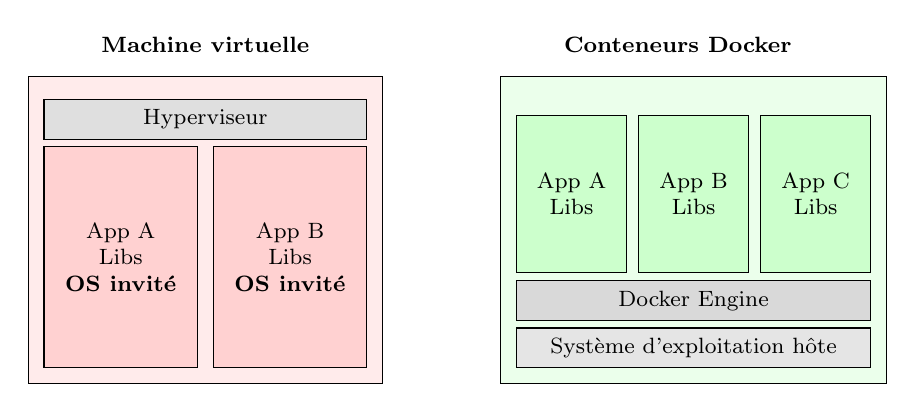
\begin{tikzpicture}[font=\footnotesize]
	% VM
	\node at (2.25,4.3) {\textbf{Machine virtuelle}};
	\draw[fill=red!8] (0,0) rectangle (4.5,3.9);
	\draw[fill=red!18] (0.2,0.2) rectangle (2.15,3.0) node[midway, align=center]{App A\\Libs\\\textbf{OS invité}};
	\draw[fill=red!18] (2.35,0.2) rectangle (4.3,3.0) node[midway, align=center]{App B\\Libs\\\textbf{OS invité}};
	\draw[fill=gray!25] (0.2,3.1) rectangle (4.3,3.6) node[midway]{Hyperviseur};
	% Conteneurs
	\node at (8.25,4.3) {\textbf{Conteneurs Docker}};
	\draw[fill=green!8] (6,0) rectangle (10.9,3.9);
	\draw[fill=green!20] (6.2,1.4) rectangle (7.6,3.4) node[midway, align=center]{App A\\Libs};
	\draw[fill=green!20] (7.75,1.4) rectangle (9.15,3.4) node[midway, align=center]{App B\\Libs};
	\draw[fill=green!20] (9.3,1.4) rectangle (10.7,3.4) node[midway, align=center]{App C\\Libs};
	\draw[fill=gray!30] (6.2,0.8) rectangle (10.7,1.3) node[midway]{Docker Engine};
	\draw[fill=gray!20] (6.2,0.2) rectangle (10.7,0.7) node[midway]{Système d'exploitation hôte};
\end{tikzpicture}
\end{center}
\noindent\textit{Figure~: la VM virtualise tout un OS, le conteneur partage le noyau hôte (plus léger).}

\newpage

\subsubsection*{Scalability}
\phantomsection
\addcontentsline{toc}{subsection}{Scalability}

La \textbf{scalabilité} (ou \textit{passage à l'échelle}) est la capacité d'un système à \textbf{absorber une augmentation de charge} (plus d'utilisateurs, plus de requêtes) en maintenant ses performances. On distingue deux stratégies~:
\begin{itemize}
	\item \textbf{Scalabilité verticale} (\textit{scale up})~: ajouter de la puissance à une même machine (plus de CPU, RAM). Simple, mais limitée et coûteuse.
	\item \textbf{Scalabilité horizontale} (\textit{scale out})~: \textbf{multiplier les instances} d'un service et répartir la charge entre elles (via un load balancer). C'est l'approche privilégiée en micro-services car elle est quasi illimitée et résiliente.
\end{itemize}
\begin{center}
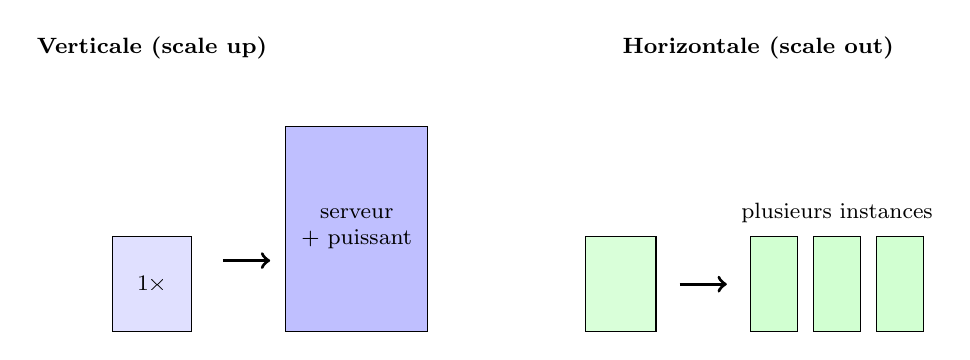
\begin{tikzpicture}[font=\footnotesize]
	% Vertical
	\node at (1.5,3.6) {\textbf{Verticale (scale up)}};
	\draw[fill=blue!12] (1.0,0) rectangle (2.0,1.2) node[midway]{1×};
	\draw[->, very thick] (2.4,0.9) -- (3.0,0.9);
	\draw[fill=blue!25] (3.2,0) rectangle (5,2.6) node[midway, align=center]{serveur\\+ puissant};
	% Horizontal
	\node at (9.2,3.6) {\textbf{Horizontale (scale out)}};
	\draw[fill=green!15] (7.0,0) rectangle (7.9,1.2) node[midway]{};
	\draw[->, very thick] (8.2,0.6) -- (8.8,0.6);
	\draw[fill=green!18] (9.1,0) rectangle (9.7,1.2);
	\draw[fill=green!18] (9.9,0) rectangle (10.5,1.2);
	\draw[fill=green!18] (10.7,0) rectangle (11.3,1.2);
	\node at (10.2,1.5) {\footnotesize plusieurs instances};
\end{tikzpicture}
\end{center}
\noindent\textit{Figure~: scalabilité verticale (machine plus puissante) vs horizontale (plus d'instances).}

\vspace{0.4cm}

\subsubsection*{CI/CD}
\phantomsection
\addcontentsline{toc}{subsection}{CI/CD}

\textbf{CI/CD} désigne une chaîne d'\textbf{automatisation} du cycle de livraison logicielle~:
\begin{itemize}
	\item \textbf{CI -- Continuous Integration} (intégration continue)~: à chaque \textit{commit}, le code est automatiquement \textbf{compilé et testé} (tests unitaires, analyse qualité), ce qui détecte les régressions au plus tôt.
	\item \textbf{CD -- Continuous Delivery / Deployment} (livraison/déploiement continu)~: les versions validées sont automatiquement \textbf{packagées} (image Docker) et \textbf{déployées} sur les environnements (test, production).
\end{itemize}
\begin{center}
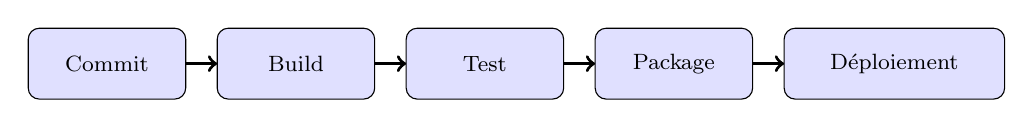
\begin{tikzpicture}[font=\footnotesize]
	\foreach \x/\t in {0/Commit, 2.4/Build, 4.8/Test, 7.2/Package} {
		\draw[fill=blue!12, rounded corners] (\x,0) rectangle (\x+2,0.9) node[midway]{\t};
	}
	\draw[fill=blue!12, rounded corners] (9.6,0) rectangle (12.4,0.9) node[midway]{Déploiement};
	\foreach \x in {2.0,4.4,6.8,9.2} { \draw[->, very thick] (\x,0.45) -- (\x+0.4,0.45); }
\end{tikzpicture}
\end{center}
\noindent\textit{Figure~: pipeline CI/CD — du commit au déploiement automatisé.}

\noindent Outils courants~: \textbf{GitHub Actions}, \textbf{GitLab CI}, \textbf{Jenkins}, \textbf{Azure DevOps}. Le CI/CD est au cœur des \textbf{bonnes pratiques de déploiement} et du \textbf{déploiement continu} visés par le projet.

\newpage

\subsubsection*{Maturité de Richardson}
\phantomsection
\addcontentsline{toc}{subsection}{Maturité de Richardson}

Le \textbf{modèle de maturité de Richardson} (\textit{Richardson Maturity Model}, RMM) est une échelle, proposée par Leonard Richardson, qui mesure à quel point une API respecte réellement les principes \textbf{REST}. Elle comporte \textbf{4 niveaux}~:
\begin{itemize}
	\item \textbf{Niveau 0 -- \og{}Le marais de POX\fg{}}~: une seule URL, un seul verbe (souvent POST), HTTP est juste un tunnel de transport (style RPC).
	\item \textbf{Niveau 1 -- Ressources}~: introduction de multiples \textbf{URI} identifiant chaque ressource (\texttt{/posts}, \texttt{/users}), mais sans usage correct des verbes.
	\item \textbf{Niveau 2 -- Verbes HTTP}~: utilisation correcte des \textbf{verbes} (GET, POST, PUT, DELETE) et des \textbf{codes de statut} (200, 404, 201…). \textbf{C'est le niveau visé par le projet} (contrainte \og{}niveau de maturité 2\fg{}) et celui de la grande majorité des API REST en production.
	\item \textbf{Niveau 3 -- HATEOAS}~: les réponses contiennent des \textbf{hyperliens} décrivant les actions possibles suivantes~; l'API devient auto-découvrable. C'est le REST \og{}pur\fg{}.
\end{itemize}
\begin{center}
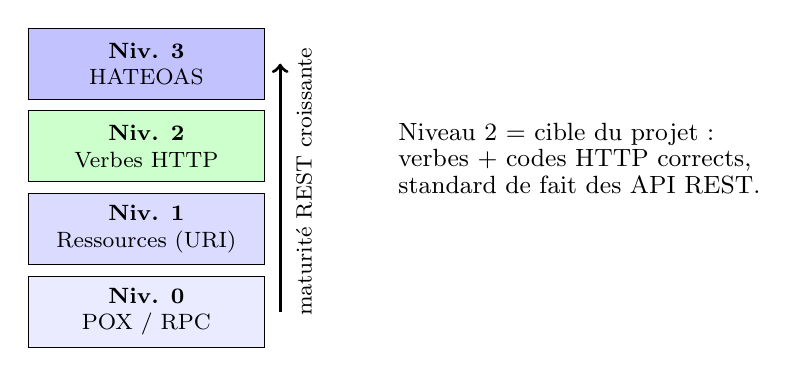
\begin{tikzpicture}[font=\footnotesize]
	\draw[fill=blue!8] (0,0) rectangle (3,0.9) node[midway, align=center]{\textbf{Niv. 0}\\POX / RPC};
	\draw[fill=blue!14] (0,1.05) rectangle (3,1.95) node[midway, align=center]{\textbf{Niv. 1}\\Ressources (URI)};
	\draw[fill=green!20] (0,2.1) rectangle (3,3.0) node[midway, align=center]{\textbf{Niv. 2}\\Verbes HTTP};
	\draw[fill=blue!24] (0,3.15) rectangle (3,4.05) node[midway, align=center]{\textbf{Niv. 3}\\HATEOAS};
	\draw[->, very thick] (3.2,0.45) -- (3.2,3.6);
	\node[rotate=90, align=center] at (3.5,2.1) {\footnotesize maturité REST croissante};
	\node[align=left] at (7.0,2.4) {\small \og{}Niveau 2\fg{} = cible du projet~:\\\small verbes + codes HTTP corrects,\\\small standard de fait des API REST.};
\end{tikzpicture}
\end{center}

\newpage

\section*{Analyse et résolution : API}
\addcontentsline{toc}{section}{Analyse et résolution : API}

\noindent \textit{Rappel de la problématique~:} \og{}Comment concevoir une API REST, scalable et intégrable dans une architecture micro-services tout en garantissant la séparation des services, la conteneurisation et la compatibilité avec une future infrastructure cloud~?\fg{}

\vspace{0.3cm}

\noindent Pour répondre, nous traitons successivement les cinq facettes de la problématique~: \textbf{(1)} le choix de l'architecture logicielle, \textbf{(2)} la conception de l'API REST et la séparation des services, \textbf{(3)} la persistance via un ORM/ODM JavaScript, \textbf{(4)} la conteneurisation, et \textbf{(5)} le déploiement et la compatibilité cloud. Une synthèse argumentée de l'architecture retenue clôt l'analyse.

\vspace{0.4cm}

\subsection*{1. Du monolithe aux micro-services~: l'architecture retenue}
\phantomsection
\addcontentsline{toc}{subsection}{1. Du monolithe aux micro-services}
\noindent Deux grandes familles d'architecture s'offraient au projet~:
\begin{itemize}
	\item \textbf{Monolithique}~: simple à démarrer, mais couplage fort, mise à l'échelle globale (on duplique \textit{tout} même pour un seul module surchargé) et re-déploiement total à chaque changement — un frein direct à la \textbf{scalabilité} et à l'\textbf{évolutivité} exigées.
	\item \textbf{Micro-services (MSA)}~: chaque capacité métier devient un service autonome, \textbf{déployé et mis à l'échelle indépendamment}, avec sa \textbf{propre base de données} (\textit{Database per Service}).
\end{itemize}
\noindent \textbf{Décision~:} l'architecture \textbf{micro-services} est retenue car elle satisfait directement les contraintes (scalabilité fine, résilience, déploiements indépendants). La migration n'est pas un \og{}Big Bang\fg{} mais \textbf{progressive} (\textit{pattern Strangler Fig})~: le \textbf{réseau social} de l'application BD est extrait en premier comme \textbf{projet pilote}, validant la démarche avant d'étendre le découpage au reste du monolithe.

\newpage

\subsection*{2. Conception de l'API REST et séparation des services}
\phantomsection
\addcontentsline{toc}{subsection}{2. Conception de l'API REST}
\noindent Le service pilote expose une \textbf{API REST} de \textbf{niveau 2 du modèle de maturité de Richardson} (contrainte projet)~: des \textbf{ressources} identifiées par des URI, manipulées par les \textbf{verbes HTTP} corrects et renvoyant les bons \textbf{codes de statut}. Pour la ressource \texttt{post}~:
\begin{center}
\begin{tabular}{|l|l|l|}
\hline
\textbf{Verbe + URI} & \textbf{Action} & \textbf{Code attendu} \\ \hline
\texttt{GET /api/posts}      & Lister les posts        & \texttt{200 OK} \\ \hline
\texttt{GET /api/posts/:id}  & Lire un post            & \texttt{200} / \texttt{404} \\ \hline
\texttt{POST /api/posts}     & Créer un post           & \texttt{201 Created} \\ \hline
\texttt{PUT /api/posts/:id}  & Mettre à jour un post   & \texttt{200} / \texttt{404} \\ \hline
\texttt{DELETE /api/posts/:id} & Supprimer un post     & \texttt{204 No Content} \\ \hline
\end{tabular}
\end{center}
\noindent La \textbf{séparation des services} est garantie par~: le caractère \textbf{sans état} (\textit{stateless}) de REST — chaque requête est autosuffisante, aucun service ne partage de session — et le principe \textit{Database per Service} qui interdit l'accès direct à la base d'un autre service. Toute communication inter-services passe par des \textbf{API REST en HTTP/JSON}, ce qui maintient un \textbf{couplage faible}.

\vspace{0.4cm}

\subsection*{3. Persistance NoSQL et ORM JavaScript (Mongoose)}
\phantomsection
\addcontentsline{toc}{subsection}{3. Persistance et ORM JavaScript}
\noindent La persistance repose sur \textbf{MongoDB} (NoSQL orienté documents) avec, comme \textbf{ORM/ODM JavaScript}, \textbf{Mongoose}. Un ODM fait le pont entre les \textbf{objets JavaScript} du code et les \textbf{documents} stockés, en évitant d'écrire des requêtes bas niveau. Concrètement, on définit un \textbf{schéma} (structure + validation), puis un \textbf{modèle} qui fournit des méthodes CRUD prêtes à l'emploi~:

\begin{minted}[fontsize=\footnotesize, bgcolor=gray!8]{javascript}
const mongoose = require('mongoose');

// 1) Schéma : structure et règles de validation du document
const postSchema = new mongoose.Schema({
  auteur:  { type: String, required: true },
  contenu: { type: String, required: true, maxlength: 500 },
  likes:   { type: Number, default: 0 },
}, { timestamps: true });            // ajoute createdAt / updatedAt

// 2) Modèle : objet manipulable offrant les opérations CRUD
const Post = mongoose.model('Post', postSchema);

\end{minted}

\newpage

\begin{minted}[fontsize=\footnotesize, bgcolor=gray!8]{javascript}
// 3) Exemple d'usage CRUD dans un contrôleur Express
async function creerPost(req, res) {
  try {
    const post = await Post.create(req.body);   // CREATE -> valide puis insère
    res.status(201).json(post);                 // 201 Created
  } catch (err) {
    res.status(400).json({ erreur: err.message }); // validation échouée
  }
}

async function listerPosts(req, res) {
  const posts = await Post.find();              // READ
  res.status(200).json(posts);
}
\end{minted}

\noindent \textbf{Apports de l'ODM dans le projet}~: \textbf{validation} automatique avant insertion (fiabilité des données), \textbf{abstraction} de l'accès aux données (code plus lisible et maintenable), méthodes CRUD (\texttt{create}, \texttt{find}, \texttt{updateOne}, \texttt{deleteOne}) qui correspondent directement aux \textbf{verbes HTTP}, et homogénéité \textbf{tout-JavaScript / JSON} du client jusqu'à la base (pile MERN). C'est la réponse concrète à l'AAV \og{}Expliquer l'utilisation d'un ORM JavaScript\fg{}.

\vspace{0.4cm}

\subsection*{4. Conteneurisation avec Docker}
\phantomsection
\addcontentsline{toc}{subsection}{4. Conteneurisation avec Docker}
\noindent Chaque micro-service est \textbf{conteneurisé} avec Docker~: il embarque l'application \textbf{et toutes ses dépendances}, garantissant une exécution \textbf{identique} du poste de développement à la production. Un \texttt{Dockerfile} décrit l'image du service~:

\begin{minted}[fontsize=\footnotesize, bgcolor=gray!8]{docker}
FROM node:20-alpine            # image légère
WORKDIR /app
COPY package*.json ./
RUN npm ci --omit=dev          # dépendances de production uniquement
COPY . .
EXPOSE 3000
CMD ["node", "server.js"]      # point d'entrée du service
\end{minted}

\noindent \textbf{Bonnes pratiques appliquées}~: image de base \textbf{Alpine} (légèreté), copie du \\ \texttt{package.json} \textbf{avant} le code pour profiter du cache de couches, \texttt{npm ci} (build reproductible), et séparation d'un conteneur par service. En développement, \textbf{Docker Compose} orchestre localement le service + une instance MongoDB.

\newpage

\subsection*{5. Propriétés non fonctionnelles}
\phantomsection
\addcontentsline{toc}{subsection}{5. Propriétés non fonctionnelles}
\noindent L'architecture retenue est évaluée au regard des \textbf{propriétés non fonctionnelles} attendues~:

\vspace{0.2cm}

\begin{center}
\begin{tabular}{|p{0.27\textwidth}|p{0.63\textwidth}|}
\hline
\textbf{Propriété} & \textbf{Comment elle est satisfaite} \\ \hline
\textbf{Fiabilité} & Validation Mongoose des données~; auto-réparation des conteneurs par l'orchestrateur. \\ \hline
\textbf{Performance} & Node.js non-bloquant~; Nginx en cache/reverse proxy~; MongoDB performant en lecture/écriture. \\ \hline
\textbf{Disponibilité} & Plusieurs instances par service~; redémarrage automatique~; load balancing. \\ \hline
\textbf{Scalabilité} & Scalabilité \textbf{horizontale} (scale out) service par service via l'orchestrateur. \\ \hline
\textbf{Connectivité} & Point d'entrée unique (API Gateway / Nginx)~; échanges normalisés HTTP/JSON. \\ \hline
\textbf{Évolutivité} & Services déployables indépendamment~; ajout d'un nouveau service sans toucher aux autres. \\ \hline
\end{tabular}
\end{center}

\vspace{0.4cm}

\subsection*{6. Infrastructures de déploiement et compatibilité cloud}
\phantomsection
\addcontentsline{toc}{subsection}{6. Déploiement et compatibilité cloud}
\noindent On distingue plusieurs \textbf{types d'infrastructures de déploiement}~:
\begin{itemize}
	\item \textbf{On-premise} (serveurs de l'entreprise)~: contrôle total, mais élasticité limitée.
	\item \textbf{IaaS} (machines virtuelles dans le cloud, ex.~AWS EC2)~: souplesse, on gère l'OS.
	\item \textbf{PaaS} (plateforme managée)~: on ne gère que l'application.
	\item \textbf{Conteneurs orchestrés} (Kubernetes / \textbf{AWS EKS})~: déploiement, scaling et résilience automatisés — \textbf{cible du projet}.
	\item \textbf{Serverless} (FaaS)~: exécution à la demande, sans serveur à gérer.
\end{itemize}
\noindent \textbf{Bonnes pratiques de déploiement d'API REST Node.js}~: variables d'environnement pour la configuration (pas de secret en dur), pipeline \textbf{CI/CD} (build → test → image Docker → déploiement), versionnement de l'API (\texttt{/api/v1}), journalisation et \textit{health checks}, et déploiements progressifs (\textit{rolling updates}) sans interruption. La conteneurisation rend l'application \textbf{portable}~: la même image tourne en local (Docker Compose) puis sur \textbf{EKS}, assurant la \textbf{compatibilité avec la future infrastructure cloud} sans réécriture.

\vspace{0.4cm}

\subsection*{7. Architecture logicielle retenue (schéma argumenté)}
\phantomsection
\addcontentsline{toc}{subsection}{7. Architecture retenue}
\noindent L'architecture cible combine tous les éléments précédents~: les clients passent par une \textbf{API Gateway / Nginx} (point d'entrée unique, routage, load balancing), qui distribue les requêtes vers des \textbf{micro-services conteneurisés}, chacun disposant de sa \textbf{propre base MongoDB}, le tout orchestré sur \textbf{AWS EKS}.
\begin{center}
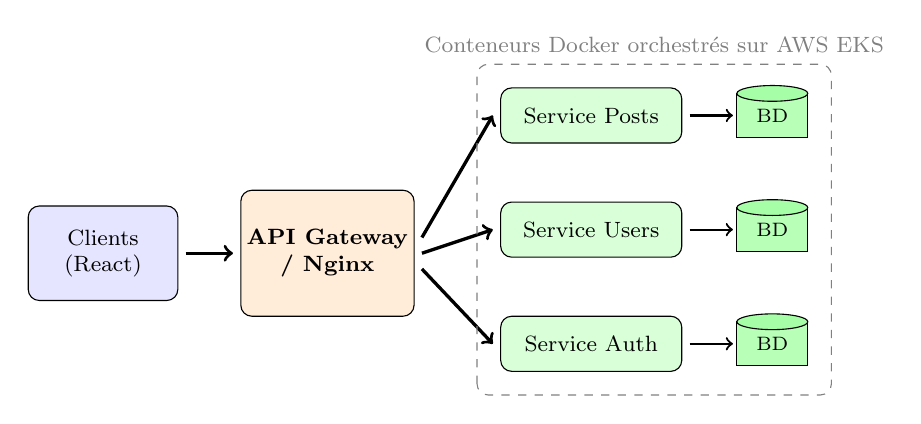
\begin{tikzpicture}[font=\footnotesize]
	\draw[fill=blue!10, rounded corners] (0,1.3) rectangle (1.9,2.5) node[midway, align=center]{Clients\\(React)};
	\draw[fill=orange!15, rounded corners] (2.7,1.1) rectangle (4.9,2.7) node[midway, align=center]{\textbf{API Gateway}\\\textbf{/ Nginx}};
	\draw[->, very thick] (2.0,1.9) -- (2.6,1.9);
	% services + bases
	\draw[fill=green!15, rounded corners] (6.0,3.3) rectangle (8.3,4.0) node[midway]{Service Posts};
	\draw[fill=green!15, rounded corners] (6.0,1.85) rectangle (8.3,2.55) node[midway]{Service Users};
	\draw[fill=green!15, rounded corners] (6.0,0.4) rectangle (8.3,1.1) node[midway]{Service Auth};
	\draw[->, very thick] (5.0,2.1) -- (5.9,3.65);
	\draw[->, very thick] (5.0,1.9) -- (5.9,2.2);
	\draw[->, very thick] (5.0,1.7) -- (5.9,0.75);
	% databases
	\foreach \y in {3.65,2.2,0.75} {
		\draw[fill=green!28] (9.0,\y-0.28) rectangle (9.9,\y+0.28);
		\draw[fill=green!35] (9.45,\y+0.28) ellipse (0.45 and 0.1);
		\node at (9.45,\y) {\scriptsize BD};
		\draw[->, thick] (8.4,\y) -- (8.95,\y);
	}
	% englobant Docker / EKS
	\draw[dashed, gray, rounded corners] (5.7,0.1) rectangle (10.2,4.3);
	\node[gray] at (7.95,4.55) {\footnotesize Conteneurs Docker orchestrés sur AWS EKS};
\end{tikzpicture}
\end{center}
\noindent\textit{Figure~: architecture retenue — API Gateway/Nginx en façade, micro-services conteneurisés avec base par service, orchestrés sur EKS.}

\vspace{0.2cm}

\noindent \textbf{Justification}~: cette architecture répond à chaque exigence de la problématique — REST de niveau 2 (intégrabilité), \textit{Database per Service} (séparation), Docker (conteneurisation), scalabilité horizontale par l'orchestrateur, et portabilité vers le cloud via EKS.

\newpage

\subsection*{Conclusion}
\phantomsection
\addcontentsline{toc}{subsection}{Conclusion}

\noindent \textbf{En réponse à la problématique}, concevoir une API REST scalable et intégrable dans une architecture micro-services passe par un ensemble de choix cohérents et complémentaires. Le service pilote — le réseau social de l'application BD — est extrait du monolithe selon une démarche progressive (\textit{Strangler Fig}) et exposé sous forme d'une \textbf{API REST de niveau 2}, ce qui en fait une brique \textbf{intégrable} et faiblement couplée. La \textbf{séparation des services} est assurée par le caractère \textit{stateless} de REST et le principe \textit{Database per Service}, chaque micro-service possédant sa propre base \textbf{MongoDB} pilotée par l'ODM \textbf{Mongoose}, qui fiabilise et simplifie l'accès aux données.

\vspace{0.2cm}

\noindent La \textbf{conteneurisation} avec Docker garantit une exécution identique de l'environnement de développement jusqu'à la production, tandis que l'orchestration sur \textbf{AWS EKS} apporte la \textbf{scalabilité horizontale}, la \textbf{disponibilité} et la \textbf{résilience} attendues, le tout exposé derrière une \textbf{API Gateway / Nginx} faisant office de point d'entrée unique et d'équilibreur de charge. Parce que l'image conteneurisée est portable, la \textbf{compatibilité avec la future infrastructure cloud} est acquise sans réécriture.

\vspace{0.2cm}

\noindent Au final, l'architecture micro-services retenue satisfait l'ensemble des propriétés non fonctionnelles visées (fiabilité, performance, disponibilité, scalabilité, connectivité, évolutivité) et constitue un \textbf{modèle reproductible}~: la démarche validée sur ce projet pilote pourra être étendue, service après service, au reste de l'application monolithique de l'entreprise.

\newpage

\section*{Capitalisation}
\addcontentsline{toc}{section}{Capitalisation}

\begin{center}
\setlength{\tabcolsep}{10pt}

\begin{tabular}{|p{0.30\textwidth}|p{0.45\textwidth}|m{0.08\textwidth}|}
\hline
\textbf{AAV} & \textbf{Commentaire} & \textbf{Statut} \\ \hline

Citer les bonnes pratiques de déploiement d'API REST en utilisant Node.js &
Bonnes pratiques détaillées~: variables d'environnement, CI/CD, versionnement d'API, \textit{health checks}, \textit{rolling updates}, image Docker portable. &
{\color{green!60!black}Acquis} \\ \hline

Citer les différents types d'infrastructures de déploiement &
On-premise, IaaS (EC2), PaaS, conteneurs orchestrés (Kubernetes/EKS) et serverless présentés et comparés. &
{\color{green!60!black}Acquis} \\ \hline

Définir les propriétés non fonctionnelles (fiabilité, performance, disponibilité, scalabilité, connectivité, évolutivité) &
Les six propriétés sont définies et reliées, via un tableau, aux choix d'architecture qui les satisfont. &
{\color{green!60!black}Acquis} \\ \hline

Expliquer l'utilisation d'un ORM JavaScript &
Rôle d'un ODM (Mongoose) expliqué~: schéma, validation, modèle et CRUD, illustré par un exemple de code commenté. &
{\color{green!60!black}Acquis} \\ \hline

Expliquer les possibilités d'architecture logicielle adaptée pour le projet (monolithique → micro-services) &
Comparaison monolithe / micro-services argumentée~; migration progressive (\textit{Strangler Fig}) et projet pilote justifiés. &
{\color{green!60!black}Acquis} \\ \hline

Représenter l'architecture logicielle retenue de manière argumentée &
Architecture cible schématisée (API Gateway/Nginx, micro-services conteneurisés, base par service, EKS) et justifiée point par point. &
{\color{green!60!black}Acquis} \\ \hline

\end{tabular}
\end{center}

\newpage

\section*{Ressources}
\addcontentsline{toc}{section}{Ressources}

\begin{itemize}
	\item \textbf{Documentation Node.js} : \url{https://nodejs.org/docs/latest/api/}
	\item \textbf{Documentation Express} : \url{https://expressjs.com/fr/}
	\item \textbf{Documentation MongoDB} : \url{https://www.mongodb.com/docs/}
	\item \textbf{Documentation Mongoose (ODM)} : \url{https://mongoosejs.com/docs/}
	\item \textbf{REST / maturité de Richardson} : \url{https://martinfowler.com/articles/richardsonMaturityModel.html}
	\item \textbf{Documentation Docker} : \url{https://docs.docker.com/}
	\item \textbf{Amazon EKS (Kubernetes managé)} : \url{https://docs.aws.amazon.com/eks/}
	\item \textbf{Microservices (patterns)} : \url{https://microservices.io/patterns/}
\end{itemize}
